% $Header: /cvsroot/latex-beamer/latex-beamer/solutions/generic-talks/generic-ornate-15min-45min.en.tex,v 1.5 2007/01/28 20:48:23 tantau Exp $

\documentclass{beamer}

\usepackage{caption}
\captionsetup{labelformat=empty,labelsep=none,font=scriptsize}
\setlength{\abovecaptionskip}{0pt}

\usepackage{color}
%% These definitions are based on darkred at
%% http://www.december.com/html/spec/colorcmyk.html
\definecolor{darkred}{cmyk}{0, 1, 1, 0.45}

% This file is a solution template for:

% - Giving a talk on some subject.
% - The talk is between 15min and 45min long.
% - Style is ornate.



% Copyright 2004 by Till Tantau <tantau@users.sourceforge.net>.
%
% In principle, this file can be redistributed and/or modified under
% the terms of the GNU Public License, version 2.
%
% However, this file is supposed to be a template to be modified
% for your own needs. For this reason, if you use this file as a
% template and not specifically distribute it as part of a another
% package/program, I grant the extra permission to freely copy and
% modify this file as you see fit and even to delete this copyright
% notice. 


\mode<presentation>
{
  \usetheme{Warsaw}
  % or ...

  \setbeamercovered{transparent}
  % or whatever (possibly just delete it)
}


\usepackage[english]{babel}
% or whatever

\usepackage[latin1]{inputenc}
% or whatever

\usepackage{times}
\usepackage[T1]{fontenc}
% Or whatever. Note that the encoding and the font should match. If T1
% does not look nice, try deleting the line with the fontenc.


%% \title[Short Paper Title] % (optional, use only with long paper titles)
%% {Presentation Title}
%% \title[]{Initial findings}
%\subtitle {Eastern CASTNET sites, May-Sep.~2001} % (optional)

%% \author[Author, Another] % (optional, use only with lots of authors)
%% {F.~Author\inst{1} \and S.~Another\inst{2}}
%% % - Use the \inst{?} command only if the authors have different
%% %   affiliation.
%% \author[Swall et al.]{Jenise Swall\inst{1}, Ana Rappold\inst{2}, and Lucas Neas\inst{2}
% - Use the \inst{?} command only if the authors have different
%   affiliation.

%% \institute[Universities of Somewhere and Elsewhere] % (optional, but mostly needed)
%% {
%%   \inst{1}%
%%   Department of Computer Science\\
%%   University of Somewhere
%%   \and
%%   \inst{2}%
%%   Department of Theoretical Philosophy\\
%%   University of Elsewhere}
%% % - Use the \inst command only if there are several affiliations.
%% % - Keep it simple, no one is interested in your street address.
 %% \institute[VCU]
 %% {
 %%   \inst{1}%
 %%   Dept.\ of Statistical Sciences and Operations Research\\
 %%   Virginia Commonwealth University
 %%   \and
 %%   \inst{2}%
 %%   National Health and Environmental Effects Research Laboratory\\
 %%   U.S.~Environmental Protection Agency
 %% }

%% \date[Short Occasion] % (optional)
%% {Date / Occasion}
\date{Feb.\ 2020}

%% \subject{Talks}
% This is only inserted into the PDF information catalog. Can be left
% out. 



% If you have a file called "university-logo-filename.xxx", where xxx
% is a graphic format that can be processed by latex or pdflatex,
% resp., then you can add a logo as follows:

% \pgfdeclareimage[height=0.5cm]{university-logo}{university-logo-filename}
% \logo{\pgfuseimage{university-logo}}



% Delete this, if you do not want the table of contents to pop up at
% the beginning of each subsection:
\AtBeginSection[]
{
  \begin{frame}<beamer>{Outline}
    \tableofcontents[currentsection,currentsubsection]
  \end{frame}
}


% If you wish to uncover everything in a step-wise fashion, uncomment
% the following command: 

%\beamerdefaultoverlayspecification{<+->}

\useoutertheme{infolines}

\begin{document}

%% \begin{frame}
%%   \titlepage
%% \end{frame}

\begin{frame}{Outline}
  \tableofcontents
  % You might wish to add the option [pausesections]
\end{frame}


% Since this a solution template for a generic talk, very little can
% be said about how it should be structured. However, the talk length
% of between 15min and 45min and the theme suggest that you stick to
% the following rules:  

% - Exactly two or three sections (other than the summary).
% - At *most* three subsections per section.
% - Talk about 30s to 2min per frame. So there should be between about
%   15 and 30 frames, all told.


%% %%%%%%%%%%%%%%%%%%%%%%%%%%%%%%%%%%%%%%%%%%%%%%%%%%%%%%%%%%



%% %%%%%%%%%%%%%%%%%%%%%%%%%%%%%
%% Introductory material
%% \section[Background]{Background ideas and info}
\section[Initial look]{Initial look at the data}


\begin{frame}{Which taxa were included?}

  {\footnotesize
    \begin{itemize}
    \item When working with the bacteria counts, I only considered
      taxa which could be classified to the family level.
    \item In this case, many taxa could not be classified at the
      family level, so all listed taxa were considered at the outset.
    \item For each sample, we calculated the total counts of all taxa
      (was 5048 for all).  Then, we calculated the fraction of counts
      associated with each taxon.  (Fractions, not counts, were used
      in the model.)
    \item To be included in the random forest model, we require that
      a taxon makes up more than 1\% of the total counts for at least
      2 samples.
     \item This process was done separately for ribs and scapualae, so
       the taxa used in random forest models differed between the 2
       types.
    \end{itemize}
  }
  
\end{frame}



\begin{frame}{Taxa for the rib model}

  {\footnotesize
    
  \noindent  Sixteen taxa were used in the random forest model for ribs.
  
  \vspace{0.1in}

  \noindent These 16 taxa were:
  
  \vspace{0.05in}

  \begin{tabular}{ll}
    Armophorea\_unclassified & Armophorida \\
    Arthropoda\_unclassified & Choreotrichia\\
    Chromadorea\_unclassified & Chrysophyceae\_unclassified\\
    Eukaryota\_unclassified & Haptoria\\
    Hypotrichia & Intramacronucleata\_unclassified\\
    Litostomatea\_unclassified & Metakinetoplastina\_unclassified\\
    Oligohymenophorea & Oligotrichia\\
    Peronosporomycetes\_fa & Synurales\_fa
  \end{tabular}
  }

\end{frame}



\begin{frame}{Taxa for the scapula model}

  {\footnotesize
    
  \noindent  ? taxa were used in the random forest model for ribs.
  
  \vspace{0.1in}

  \noindent These were:\\
  \begin{tabular}{ll}

  \end{tabular}
  }

\end{frame}
%% %%%%%%%%%%%%%%%%%%%%%%%%%%%%%

\end{document}


%% %%%%%%%%%%%%%%%%%%%%%%%%%%%%%
\section[Henley Lake]{Analysis using Henley Lake family-level taxa}


%% %%%%%%%%%%%%%
\subsection[Ribs]{Working with rib samples}

\begin{frame}{Implementing the random forest model for ribs}

\begin{itemize}
\item The model utilized 24 family-level taxa.
\item Cross-validation was used to determine that the best number of
  taxa to consider at each "branching".  This changed very little
  whether including or omitting baseline samples.
\end{itemize}

\vspace{0.1in}

\noindent For the fitted model, using baseline samples:\\
\noindent RMSE: 517.0 $\pm$ 6.3  \hspace{0.05in}  Explained variation: 89.5\%
$\pm$ 0.3\%

\vspace{0.1in}

\noindent For the fitted model, omitting baseline samples:\\
\noindent RMSE: 538.2 $\pm$ 6.3  \hspace{0.05in}  Explained variation: 87.7\%
$\pm$ 0.3\%

\end{frame}



\begin{frame}{Influential taxa}

%  \begin{center}
  \begin{minipage}{0.47\textwidth}
    \begin{figure}
    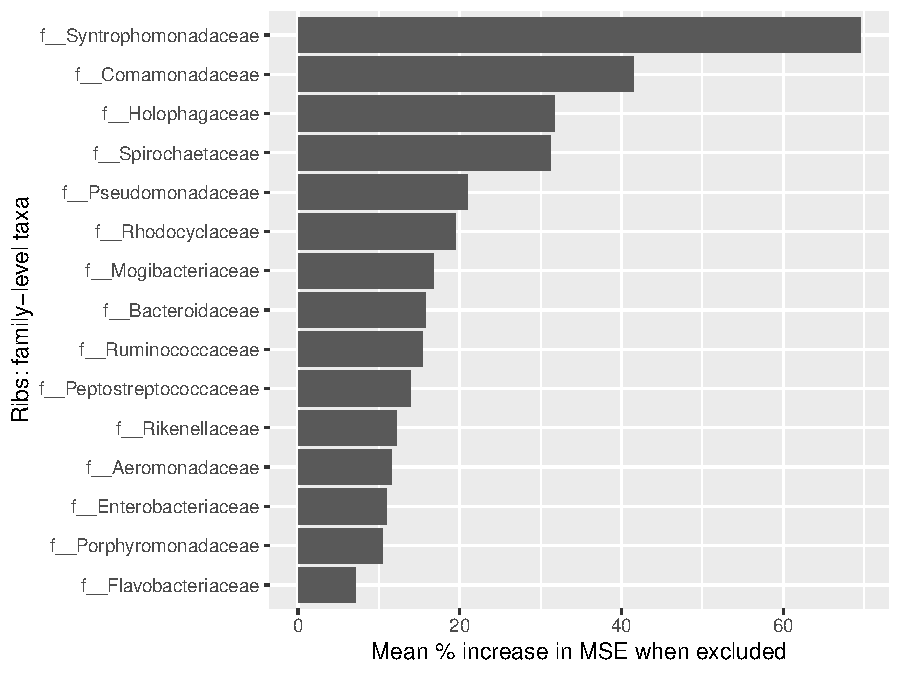
\includegraphics[width=2.25in]{HenleyLake/bacteria/use_families/w_ribs/w_baseline/families_rib_PercIncMSE_barchart}
    \caption{{\tiny Using baseline samples}}
\end{figure}
\end{minipage}
\begin{minipage}{0.47\textwidth}
  \begin{figure}
    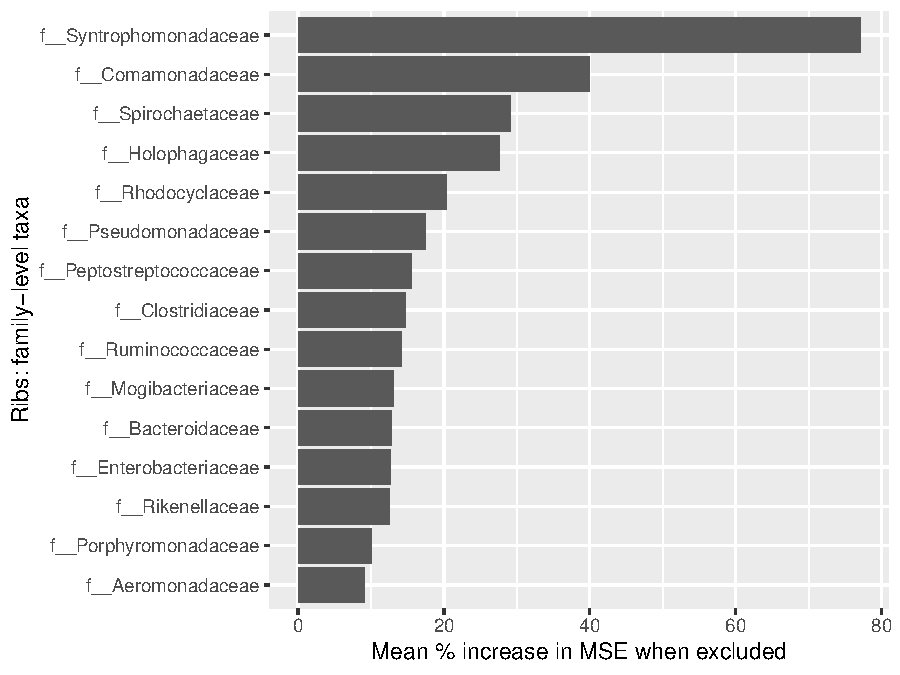
\includegraphics[width=2.25in]{HenleyLake/bacteria/use_families/w_ribs/no_baseline/families_rib_no_baseline_PercIncMSE_barchart}
    \caption{{\tiny Omitting baseline samples}}
  \end{figure}
  \end{minipage}
%  \end{center}
  \vspace{0.1in}
  {\scriptsize
  \begin{itemize}
  \item The measure of importance is the mean percentage increase in the
    mean-square error of model predictions when the variable is left out of the
    model. 
  \item I've shown the top 15 because they'd fit, but 24 were used in the model.
  \item The taxa are similar whether we include the baseline samples or not.
  \end{itemize}
  }

\end{frame}



\begin{frame}{Scatterplots for influential taxa, with baseline samples}

  \begin{center}
    \begin{figure}
      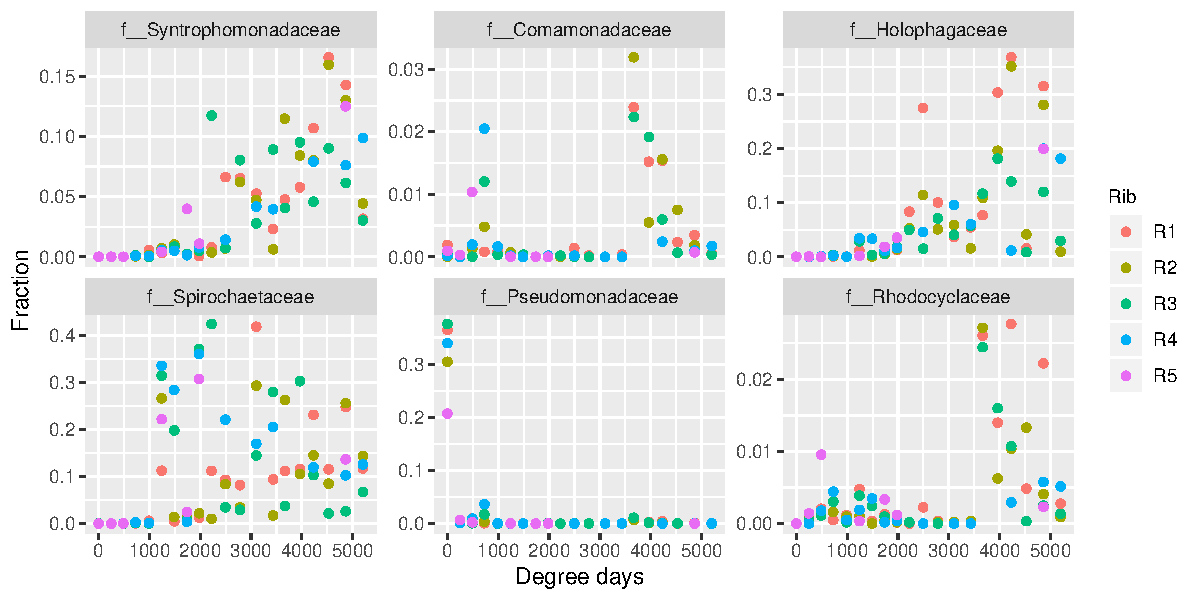
\includegraphics[width=4.75in]{HenleyLake/bacteria/use_families/w_ribs/w_baseline/infl_rib_family_scatter}
    \end{figure}
  \end{center}
  \vspace{-0.25in}
  {\scriptsize
  \begin{itemize}
  \item I've only shown top 6 because more than that is hard to fit.
  \item Note that the y-axes have differing scales.
  \item Fractions of Comamonadaceae and Rhodocyclaceae are very low.
  \end{itemize}
  }

\end{frame}


\begin{frame}{Scatterplots for influential taxa, no baseline samples}

  \begin{center}
    \begin{figure}
      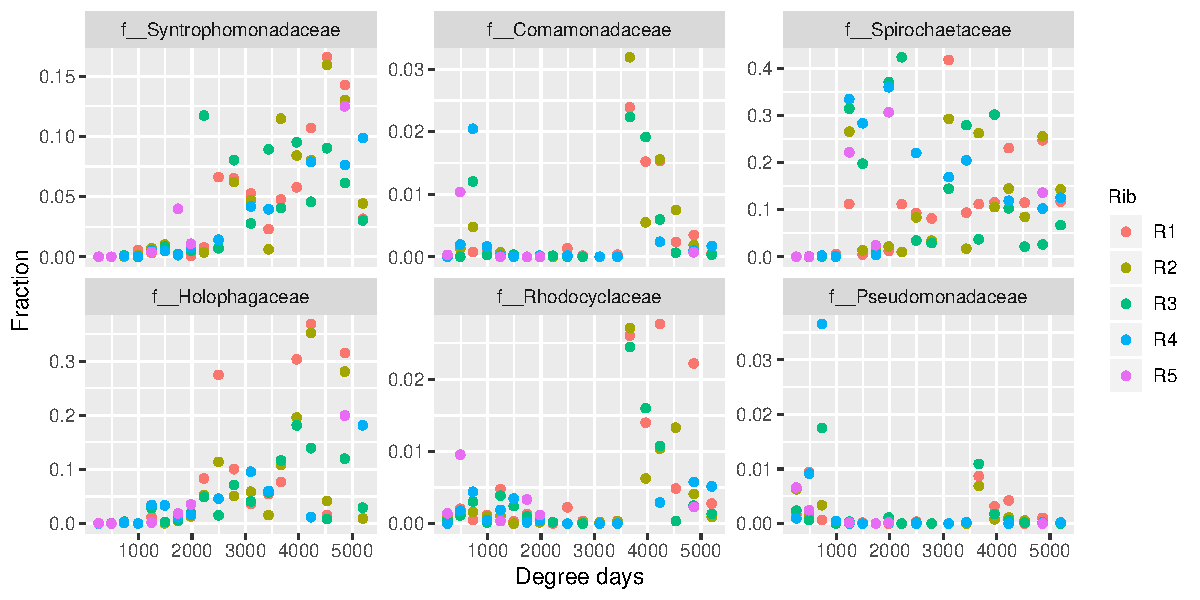
\includegraphics[width=4.75in]{HenleyLake/bacteria/use_families/w_ribs/no_baseline/infl_rib_family_no_baseline_scatter}
    \end{figure}
  \end{center}
  \vspace{-0.25in}
  {\scriptsize
  \begin{itemize}
  \item These are the same six taxa as the analysis with baseline samples, though in a slightly changed order.
  \end{itemize}
  }

\end{frame}



\begin{frame}{Getting a sense of "real-life" model fit}

  \noindent In real life, we would be estimating ADD without
  \begin{itemize}
    \item having seen that rib/scapula before, and
    \item maybe not having observed any rib/scapula at that level of ADD before
  \end{itemize} 

  \vspace{0.1in}

  \noindent To try to get a sense of how the model would work in such cases, I
  \begin{itemize}
    \item fitted the model over and over, each time without one particular
    combination of rib/scapula number and ADD.
    \item This means the model had no info about the left-out rib/scapula and no
    info about bacteria counts at that ADD.
    \item Then, I used the model to estimate the ADD for the left-out
    rib/scapula for the left-out ADD.
  \end{itemize}
  
\end{frame}


\begin{frame}{Residual plot to get sense of "real-life" model fit}

  \begin{minipage}{0.47\textwidth}
  \begin{figure}
      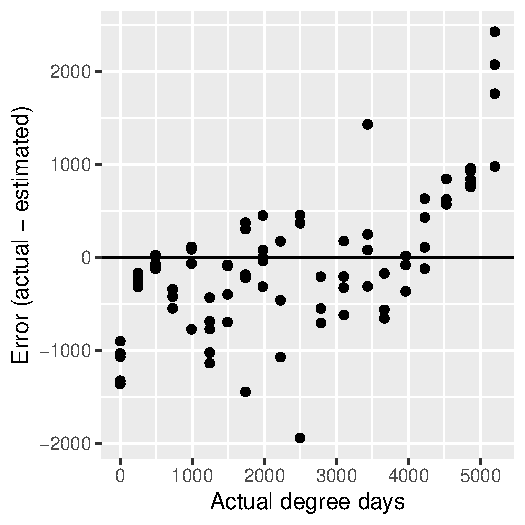
\includegraphics[width=1.5in]{HenleyLake/bacteria/use_families/w_ribs/w_baseline/leave_out_one_rib_and_one_day_residuals}
      \caption{With baseline samples}
  \end{figure}
  \end{minipage}  
  \begin{minipage}{0.47\textwidth}
  \begin{figure}
      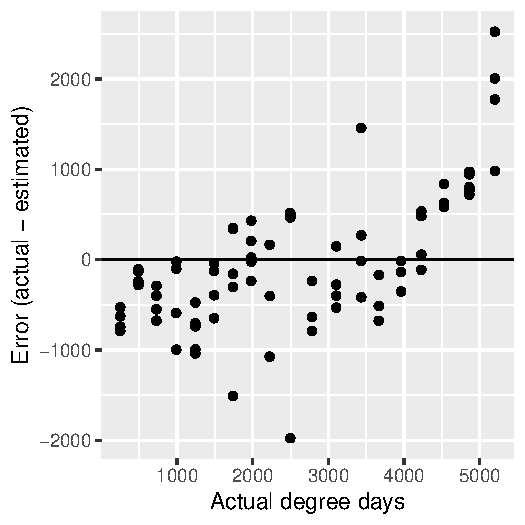
\includegraphics[width=1.5in]{HenleyLake/bacteria/use_families/w_ribs/no_baseline/leave_out_one_rib_and_one_day_residuals}
      \caption{Omitting baseline samples}
  \end{figure}
  \end{minipage}
    \vspace{0.1in}
{\scriptsize
\begin{itemize}
  \item This RMSE is in the range of 741-744 for both, which is
    higher than the RMSE for the full dataset (as you'd expect).  We
    have less data available for each run, and we're predicting for an
    ADD value which we have no information about.
  \item The errors tend to be larger at the extremes.
\end{itemize}
}

\end{frame}
%% %%%%%%%%%%%%%



%% %%%%%%%%%%%%%
\subsection[Scapulae]{Working with scapula samples}

\begin{frame}{Implementing the random forest model for scapulae}

\begin{itemize}
\item The model utilized 34 family-level taxa.
\item Cross-validation was used to determine that the best number of
  taxa to consider at each "branching".  This changed very little
  whether including or omitting baseline samples.
\end{itemize}

\vspace{0.1in}

\noindent For the fitted model, using baseline samples:\\
\noindent RMSE: 334.2 $\pm$ 4.4  \hspace{0.05in}  Explained variation: 95.3\%
$\pm$ 0.1\%

\vspace{0.1in}

\noindent For the fitted model, omitting baseline samples:\\
\noindent RMSE: 331.9 $\pm$ 4.5  \hspace{0.05in}  Explained variation: 95.2\%
$\pm$ 0.1\%

\end{frame}



\begin{frame}{Influential taxa}

  \begin{minipage}{0.47\textwidth}
    \begin{figure}
    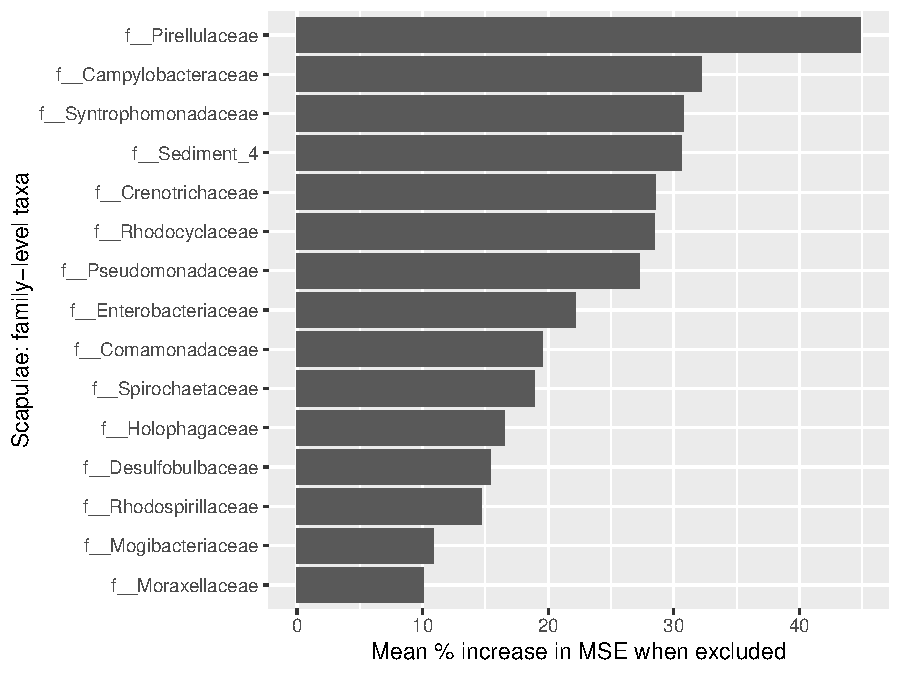
\includegraphics[width=2.25in]{HenleyLake/bacteria/use_families/w_scapulae/w_baseline/families_scapula_PercIncMSE_barchart}
    \caption{Using baseline samples}
\end{figure}
\end{minipage}
\begin{minipage}{0.47\textwidth}
  \begin{figure}
    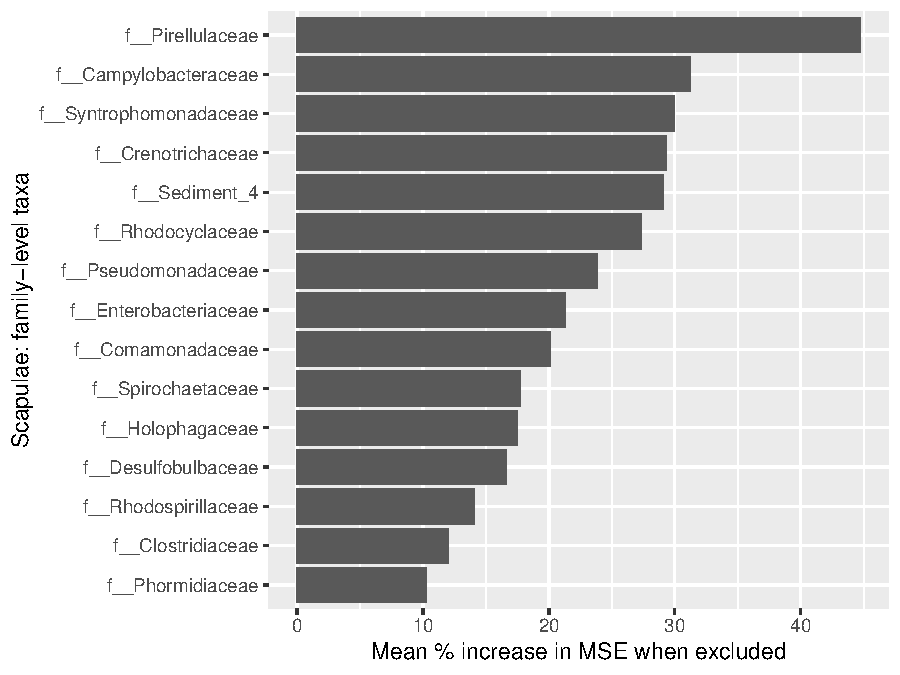
\includegraphics[width=2.25in]{HenleyLake/bacteria/use_families/w_scapulae/no_baseline/families_scapula_no_baseline_PercIncMSE_barchart}
    \caption{Omitting baseline samples}
  \end{figure}
  \end{minipage}
%  \end{center}
  \vspace{0.1in}
  {\scriptsize
  \begin{itemize}
  \item Again, I've just shown the top 15.
  \item The taxa are similar whether we include the baseline samples or not.
  \end{itemize}
  }

\end{frame}



\begin{frame}{Scatterplots for influential taxa, with baseline samples}

  \begin{center}
    \begin{figure}
      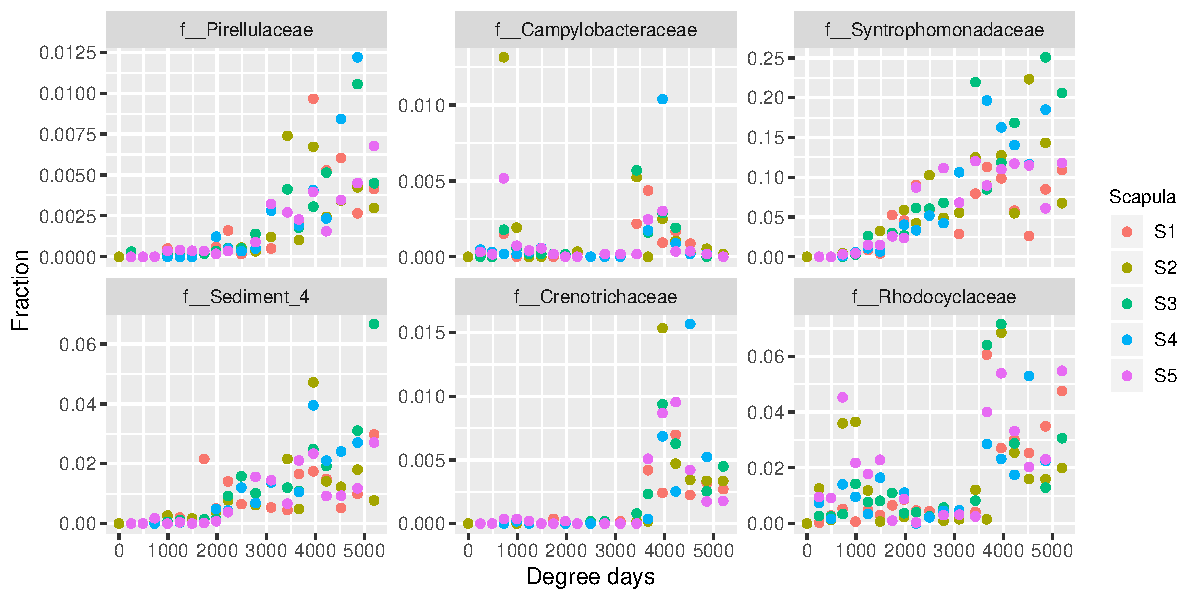
\includegraphics[width=4.75in]{HenleyLake/bacteria/use_families/w_scapulae/w_baseline/infl_scapula_family_scatter}
    \end{figure}
  \end{center}
  \vspace{-0.25in}
  {\scriptsize
  \begin{itemize}
  \item Again, I've only shown top 6.
  \item Note that the y-axes have differing scales.
  \item Fractions of Pirellulaceae, Campylobacteraceae, and Crenotrichacea
  are very low.
  \end{itemize}
  }

\end{frame}



\begin{frame}{Scatterplots for influential taxa, no baseline samples}

  \begin{center}
    \begin{figure}
      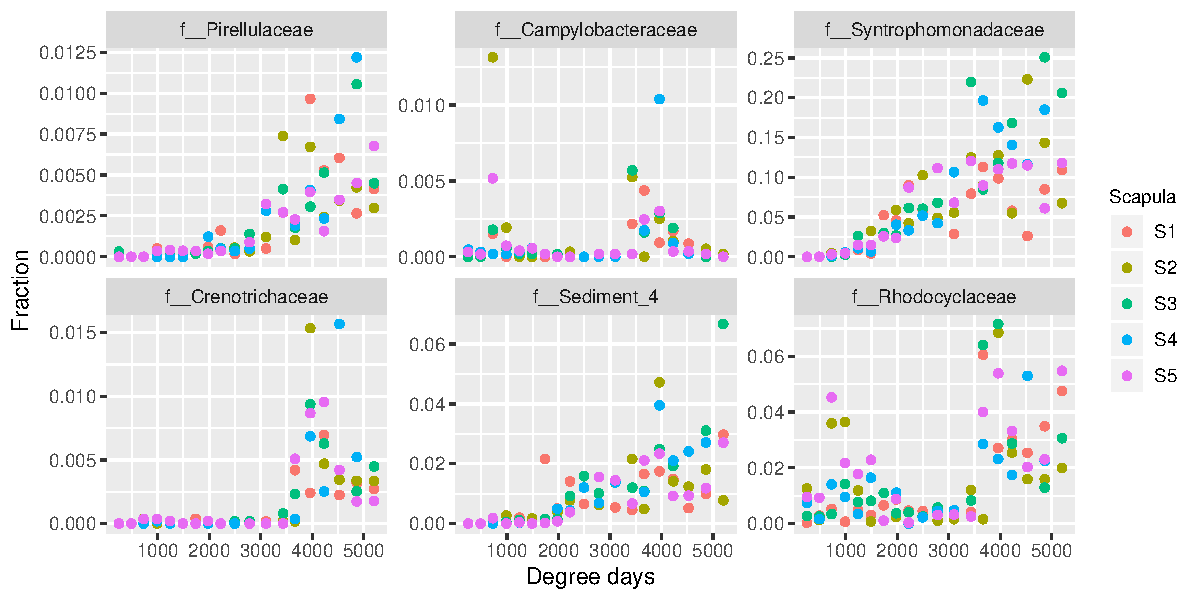
\includegraphics[width=4.75in]{HenleyLake/bacteria/use_families/w_scapulae/no_baseline/infl_scapula_family_no_baseline_scatter}
    \end{figure}
  \end{center}
  \vspace{-0.25in}
  {\scriptsize
  \begin{itemize}
  \item These are the same six taxa as the analysis with baseline samples, though in a slightly changed order.
  \end{itemize}
  }

\end{frame}




\begin{frame}{Residual plot to get sense of "real-life" model fit}

  \begin{minipage}{0.47\textwidth}
  \begin{figure}
      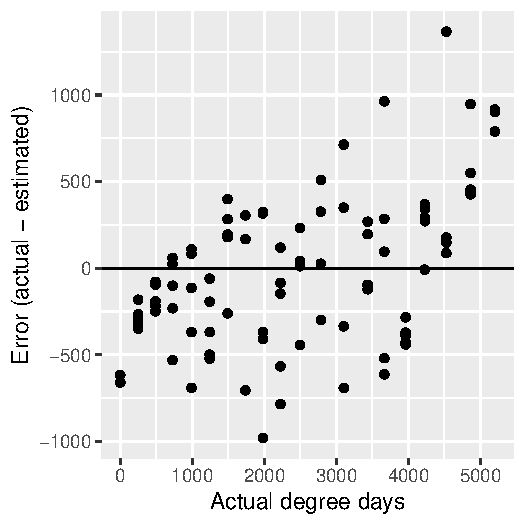
\includegraphics[width=1.5in]{HenleyLake/bacteria/use_families/w_scapulae/w_baseline/leave_out_one_scapula_and_one_day_residuals}
      \caption{With baseline samples}
  \end{figure}
  \end{minipage}  
  \begin{minipage}{0.47\textwidth}
  \begin{figure}
      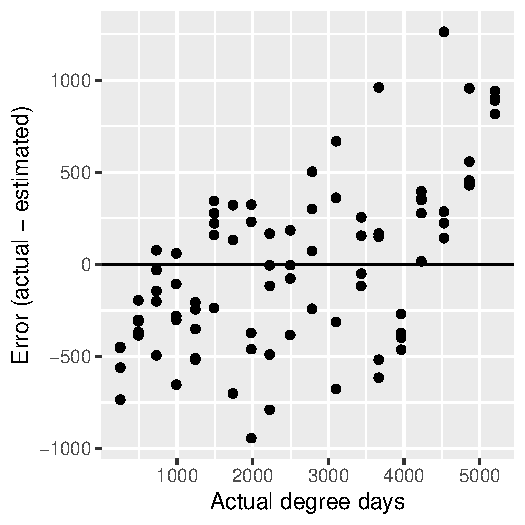
\includegraphics[width=1.5in]{HenleyLake/bacteria/use_families/w_scapulae/no_baseline/leave_out_one_scapula_and_one_day_residuals}
      \caption{Omitting baseline samples}
  \end{figure}
  \end{minipage}
    \vspace{0.1in}
{\scriptsize
\begin{itemize}
\item The RMSE is in the range of 450-453 when we include baseline observations.
\item The RMSE is in the range of 459-461 when we omit baseline observations.
\end{itemize}
}

\end{frame}
%% %%%%%%%%%%%%%
%% %%%%%%%%%%%%%%%%%%%%%%%%%%%%%




%% %%%%%%%%%%%%%%%%%%%%%%%%%%%%%
\section[Rice Rivers]{Analysis using Rice Rivers family-level taxa}


%% %%%%%%%%%%%%%
\subsection[Ribs]{Working with rib samples}

\begin{frame}{Implementing the random forest model for ribs}

\begin{itemize}
\item The model utilized 41 family-level taxa, which is many more taxa
  than we used for the Henley Lake analysis.
\item Cross-validation was used to determine that the best number of
  taxa to consider at each "branching".  The number of taxa to
  consider was slightly lower when we omitted the baseline samples.
\end{itemize}

\vspace{0.1in}

\noindent For the fitted model, using baseline samples:\\
\noindent RMSE: 475.1 $\pm$ 5.6  \hspace{0.05in}  Explained variation: 93.6\%
$\pm$ 0.1\%

\vspace{0.1in}

\noindent For the fitted model, omitting baseline samples:\\
\noindent RMSE: 476.6 $\pm$ 5.7  \hspace{0.05in}  Explained variation: 93.2\%
$\pm$ 0.2\%

\end{frame}



\begin{frame}{Influential taxa}

  \begin{minipage}{0.47\textwidth}
    \begin{figure}
      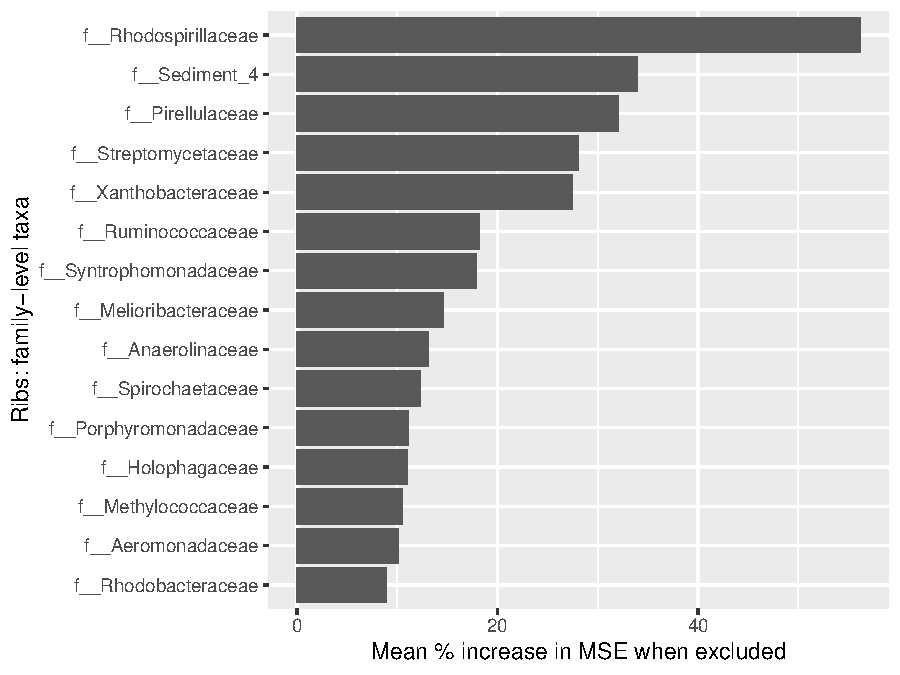
\includegraphics[width=2.25in]{RiceRivers/bacteria/use_families/w_ribs/w_baseline/families_rib_w_baseline_PercIncMSE_barchart}
      \caption{Using baseline samples}
    \end{figure}
  \end{minipage}
  \begin{minipage}{0.47\textwidth}
    \begin{figure}
      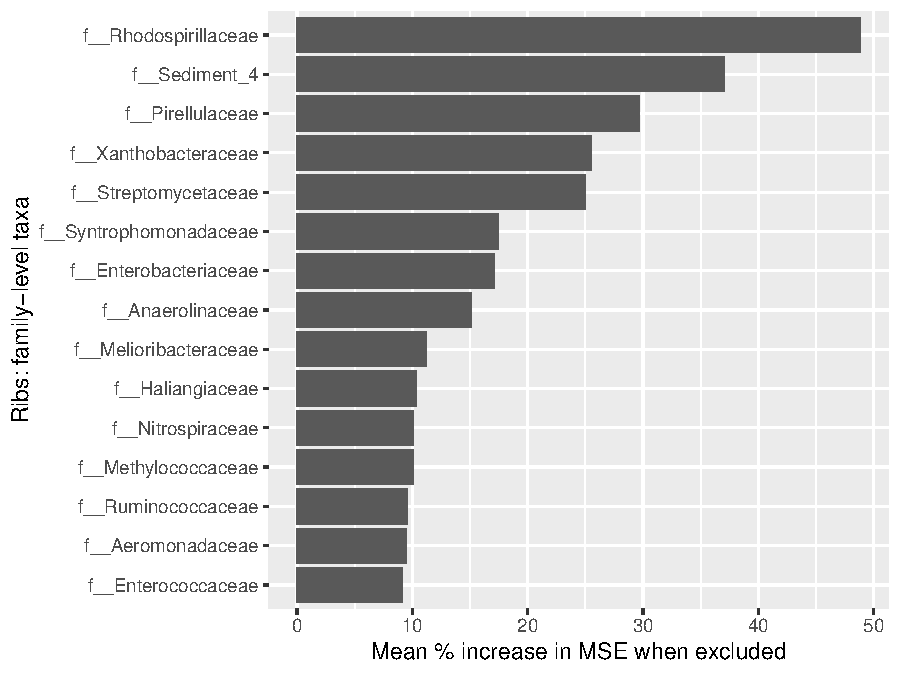
\includegraphics[width=2.25in]{RiceRivers/bacteria/use_families/w_ribs/no_baseline/families_rib_no_baseline_PercIncMSE_barchart}
      \caption{Omitting baseline samples}
    \end{figure}
  \end{minipage}
  \vspace{0.1in}
  {\scriptsize
  \begin{itemize}
  \item Most of taxa identified as most influential are the same.  The top 5 are the same in both cases, though in slightly different orders.
  \item There are more differences from the 6th most influential on down.
  \end{itemize}
  }

\end{frame}



\begin{frame}{Scatterplots for influential taxa, with baseline samples}

  \begin{center}
    \begin{figure}
      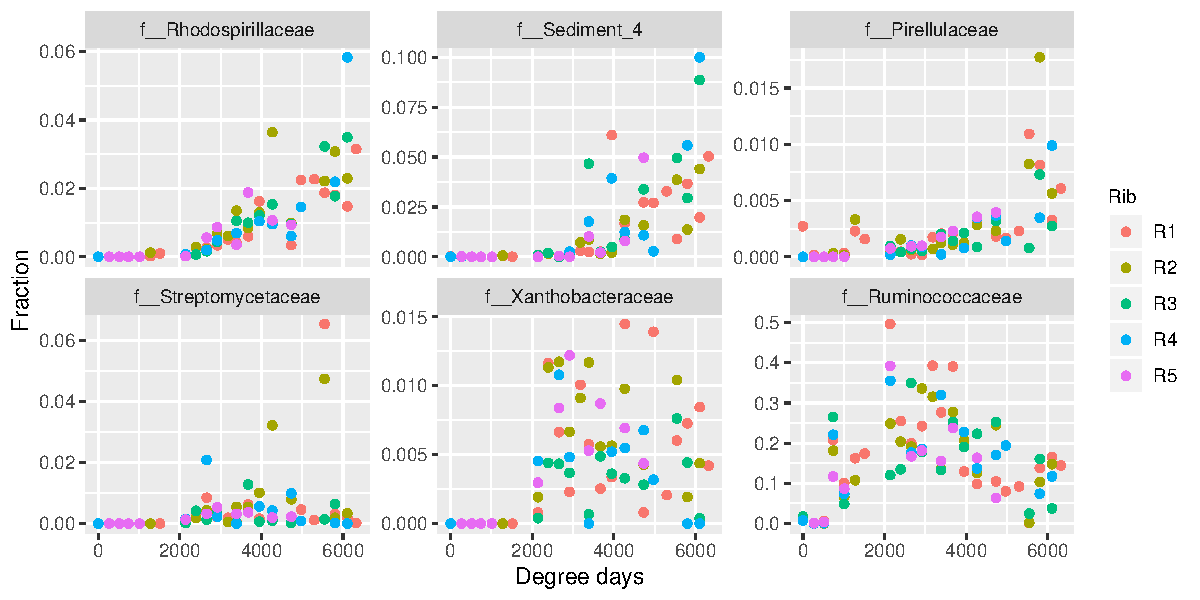
\includegraphics[width=4.75in]{RiceRivers/bacteria/use_families/w_ribs/w_baseline/infl_rib_family_w_baseline_scatter}
    \end{figure}
  \end{center}
  \vspace{-0.25in}
  {\scriptsize
  \begin{itemize}
  \item Again, I've only shown top 6 because more than that is hard to fit.
  \item Note that the y-axes have differing scales.
  \item Fractions of Pirellulaceae and Xanthobacteraceae are very low.
  \end{itemize}
  }

\end{frame}



\begin{frame}{Scatterplots for influential taxa, no baseline samples}

  \begin{center}
    \begin{figure}
      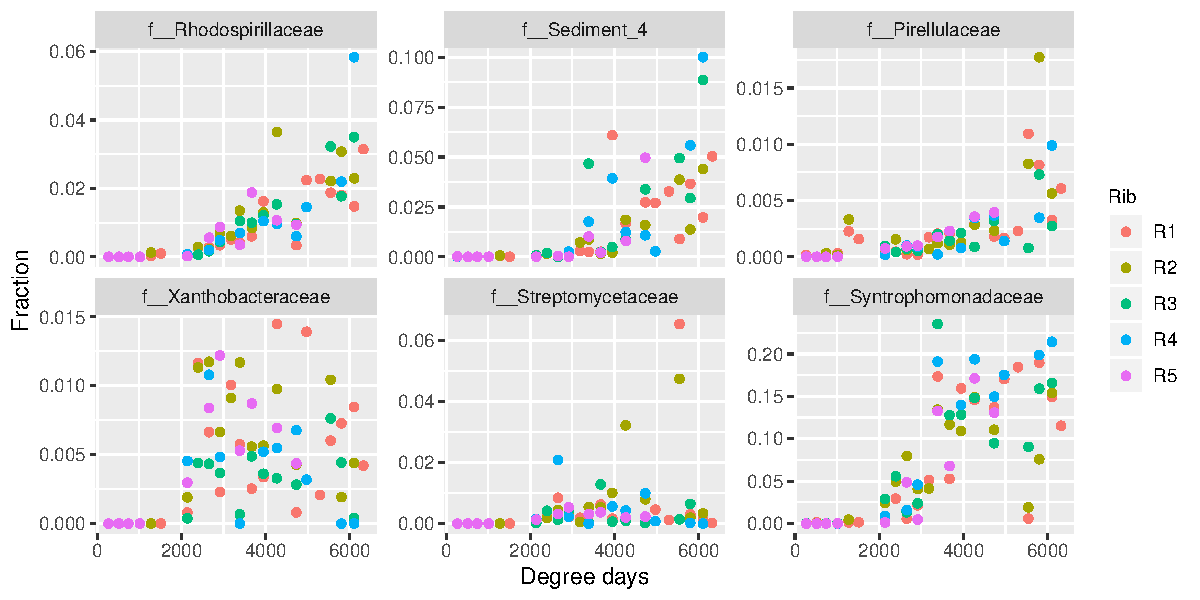
\includegraphics[width=4.75in]{RiceRivers/bacteria/use_families/w_ribs/no_baseline/infl_rib_family_no_baseline_scatter}
    \end{figure}
  \end{center}
  \vspace{-0.25in}
  {\scriptsize
  \begin{itemize}
  \item The sixth taxa is different between the analysis with and without the baseline samples.
  \end{itemize}
  }

\end{frame}



\begin{frame}{Residual plot to get sense of "real-life" model fit}

  \begin{minipage}{0.47\textwidth}
  \begin{figure}
      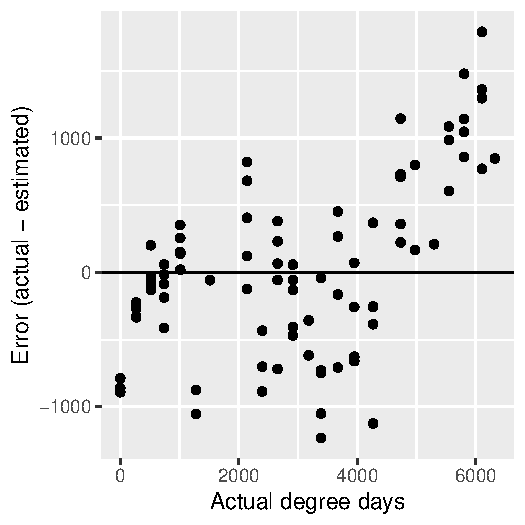
\includegraphics[width=1.5in]{RiceRivers/bacteria/use_families/w_ribs/w_baseline/leave_out_one_rib_and_one_day_residuals}
      \caption{With baseline samples}
  \end{figure}
  \end{minipage}  
  \begin{minipage}{0.47\textwidth}
  \begin{figure}
      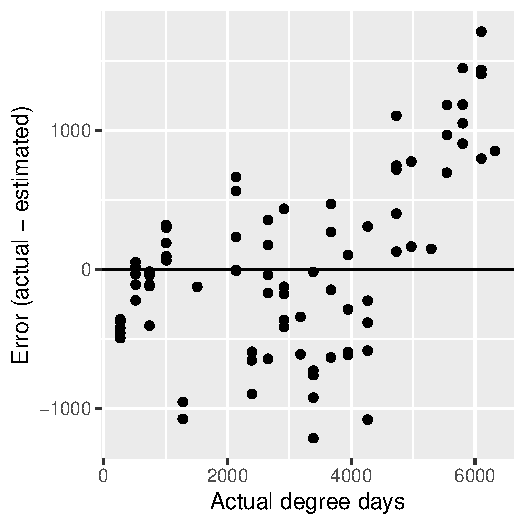
\includegraphics[width=1.5in]{RiceRivers/bacteria/use_families/w_ribs/no_baseline/leave_out_one_rib_and_one_day_residuals}
      \caption{Omitting baseline samples}
  \end{figure}
  \end{minipage}
    \vspace{0.1in}
{\scriptsize
  \begin{itemize}
  \item The RMSE is in the range of 651-655 when using baseline samples.
  \item The RMSE is in the range of 645-648 when baseline samples are omitted.
  \end{itemize}
}

\end{frame}
%% %%%%%%%%%%%%%



%% %%%%%%%%%%%%%
\subsection[Scapulae]{Working with scapula samples}

\begin{frame}{Implementing the random forest model for scapulae}

\begin{itemize}
\item The model utilized 55 family-level taxa.
\item Cross-validation was used to determine that the best number of
  taxa to consider at each "branching".  This was the same whether
  including or omitting baseline samples.
\end{itemize}

\vspace{0.1in}

\noindent For the fitted model, using baseline samples:\\
\noindent RMSE: 501.1 $\pm$ 5.1  \hspace{0.05in}  Explained variation: 93.3\%
$\pm$ 0.1\%

\vspace{0.1in}

\noindent For the fitted model, omitting baseline samples:\\
\noindent RMSE: 506.4 $\pm$ 5.1  \hspace{0.05in}  Explained variation: 92.6\%
$\pm$ 0.1\%

\end{frame}



\begin{frame}{Influential taxa}

  \begin{minipage}{0.47\textwidth}
    \begin{figure}
    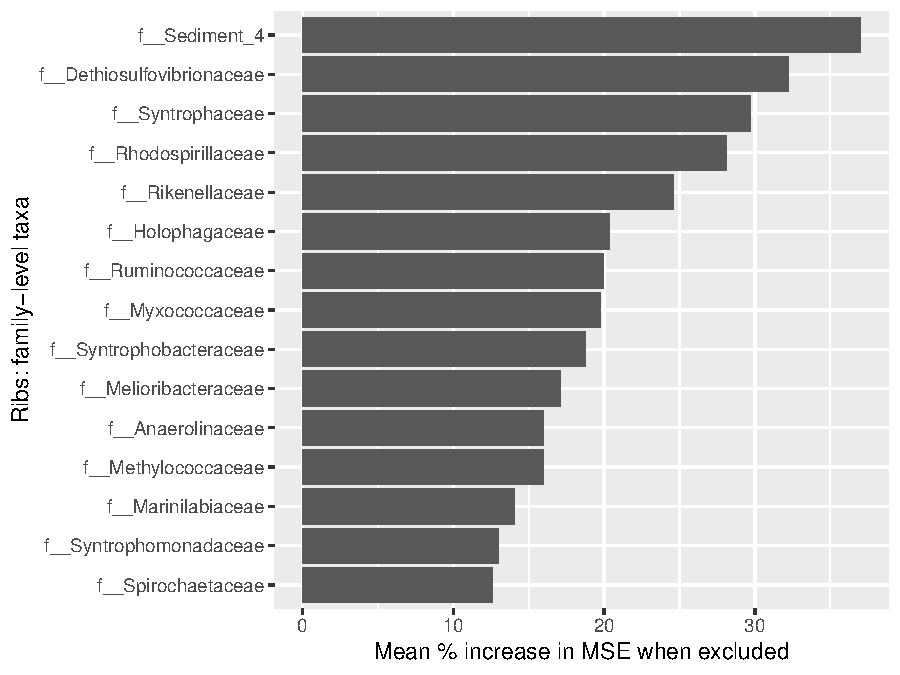
\includegraphics[width=2.25in]{RiceRivers/bacteria/use_families/w_scapulae/w_baseline/families_scapula_w_baseline_PercIncMSE_barchart}
    \caption{Using baseline samples}
\end{figure}
\end{minipage}
\begin{minipage}{0.47\textwidth}
  \begin{figure}
    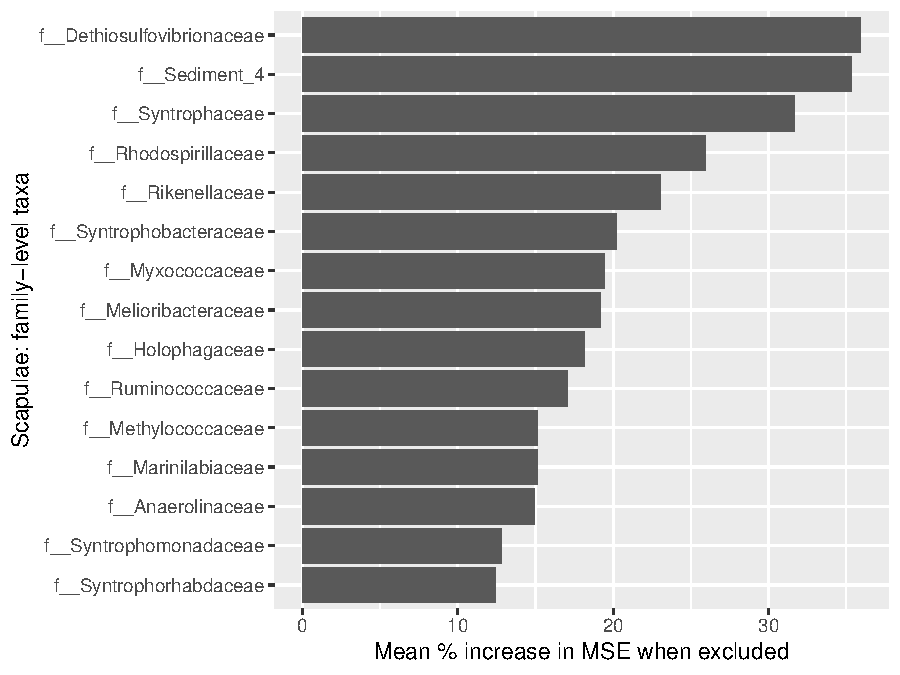
\includegraphics[width=2.25in]{RiceRivers/bacteria/use_families/w_scapulae/no_baseline/families_scap_no_baseline_PercIncMSE_barchart}
    \caption{Omitting baseline samples}
  \end{figure}
  \end{minipage}
  \vspace{0.1in}
  {\scriptsize
  \begin{itemize}
  \item The top 5 taxa are the same in both cases, though the order
    for first and second changes.
  \item There are some differences from the sixth taxa on down.
  \end{itemize}
  }

\end{frame}



\begin{frame}{Scatterplots for influential taxa, with baseline samples}

  \begin{center}
    \begin{figure}
      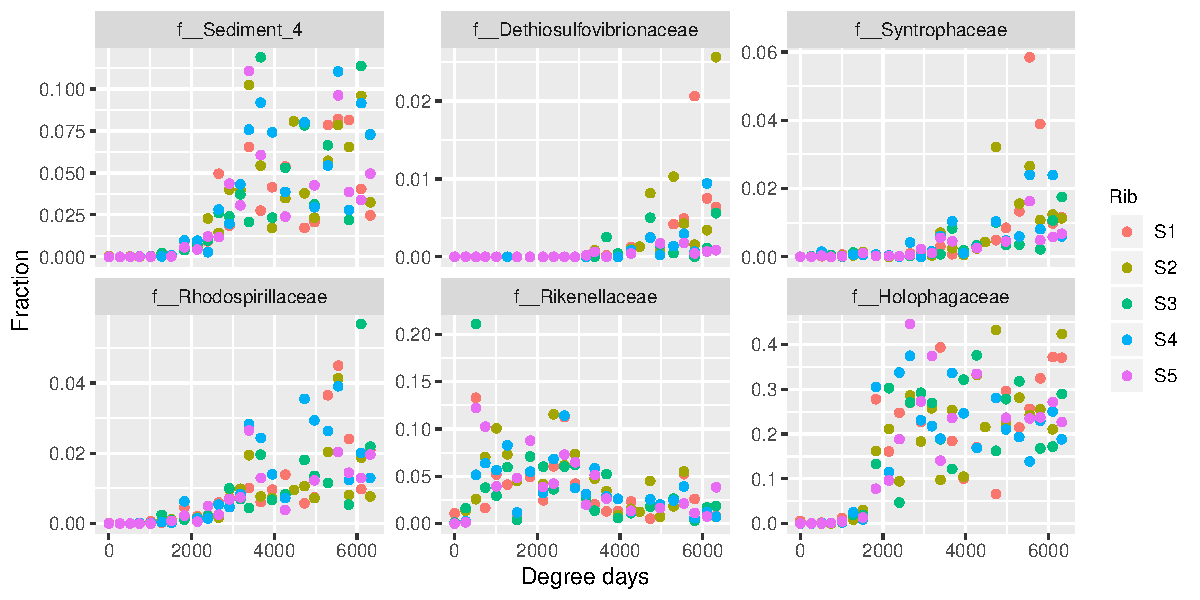
\includegraphics[width=4.75in]{RiceRivers/bacteria/use_families/w_scapulae/w_baseline/infl_scapula_family_w_baseline_scatter}
    \end{figure}
  \end{center}
  \vspace{-0.25in}
  {\scriptsize
  \begin{itemize}
  \item Again, I've only shown the top 6.
  \item None of these taxa have consistently very low fractions, which is different from some of the other analyses.
  \end{itemize}
  }

\end{frame}



\begin{frame}{Scatterplots for influential taxa, no baseline samples}

  \begin{center}
    \begin{figure}
      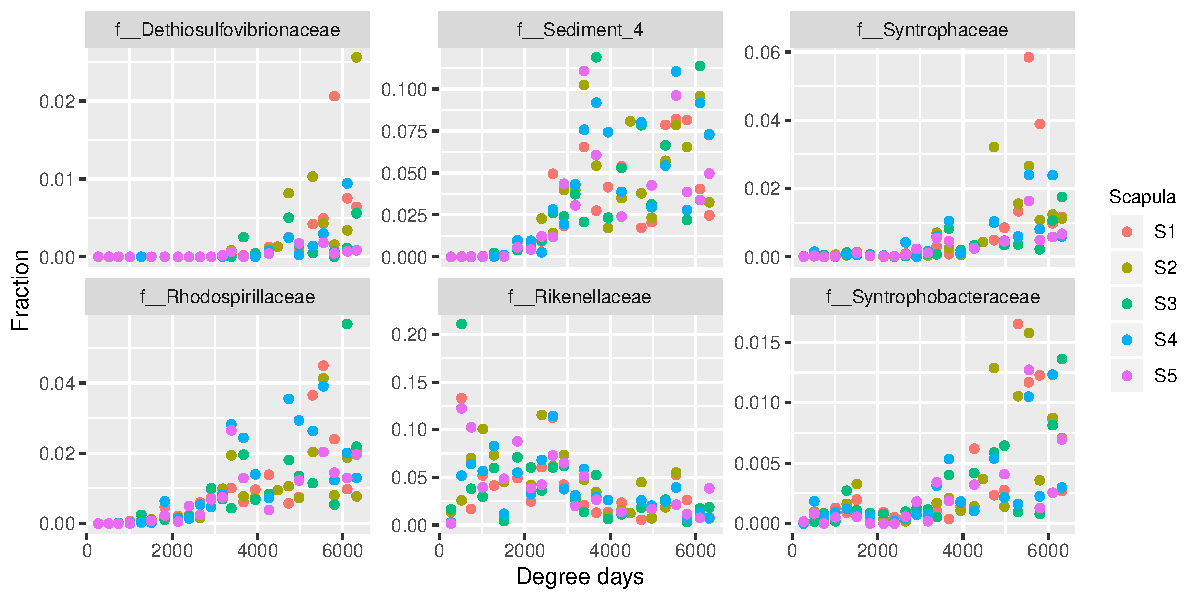
\includegraphics[width=4.75in]{RiceRivers/bacteria/use_families/w_scapulae/no_baseline/infl_scap_family_no_baseline_scatter}
    \end{figure}
  \end{center}
  \vspace{-0.25in}
  {\scriptsize
  \begin{itemize}
  \item The sixth taxa, Syntrophobacteraceae, is different from the
    analysis using the baseline samples (Holophagaceae).
    \item The fractions for Syntrophobacteraceae are consistently low.
  \end{itemize}
  }

\end{frame}



\begin{frame}{Residual plot to get sense of "real-life" model fit}

  \begin{minipage}{0.47\textwidth}
  \begin{figure}
      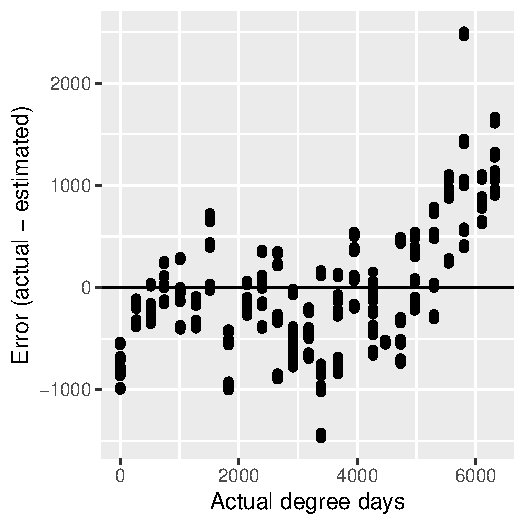
\includegraphics[width=1.5in]{RiceRivers/bacteria/use_families/w_scapulae/w_baseline/leave_out_one_scapula_and_one_day_residuals}
      \caption{With baseline samples}
  \end{figure}
  \end{minipage}  
  \begin{minipage}{0.47\textwidth}
  \begin{figure}
      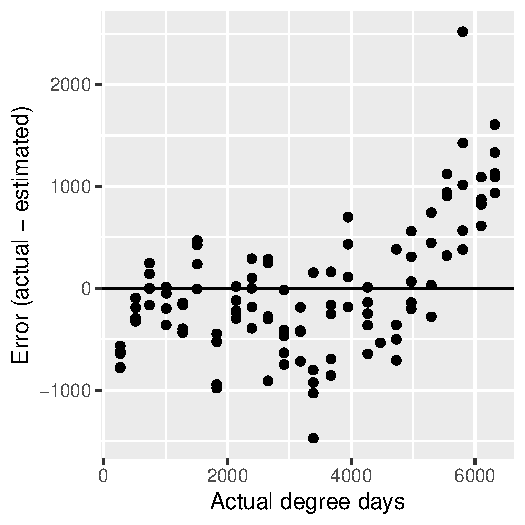
\includegraphics[width=1.5in]{RiceRivers/bacteria/use_families/w_scapulae/no_baseline/leave_out_one_scap_and_one_day_residuals}
      \caption{Omitting baseline samples}
  \end{figure}
  \end{minipage}
    \vspace{0.1in}
{\scriptsize
\begin{itemize}
\item The RMSE is in the range of 630-632 when we include baseline observations.
\item The RMSE is in the range of 637-639 when we omit baseline observations.
\end{itemize}
}

\end{frame}
%% %%%%%%%%%%%%%
%% %%%%%%%%%%%%%%%%%%%%%%%%%%%%%

\end{document}
